\documentclass{beamer}

\usepackage[utf8]{inputenc}
\usepackage{hyperref}

\usetheme{Berkeley}
\beamertemplatenavigationsymbolsempty
\setbeamertemplate{headline}{}
 
\title{Geocoding in FoodChain-Lab}
\date{}
 
\begin{document}
\maketitle

\section{ }

\subsection{Task}
\begin{frame}
	\begin{itemize}
		\item Perform a geocoding by using the Geocoding workflow from \url{https://github.com/SiLeBAT/BfROpenLabResources/raw/master/GitHubPages/workflows/Geocoding.zip}.
		\item Use "Street", "HouseNumber", "City" and "Country" as input parameters.
		\item Do the geocoding by using the MapQuest Geocoding Service.
	\end{itemize}
\end{frame}
 
\subsection{1}
\begin{frame}
	\begin{center}
  		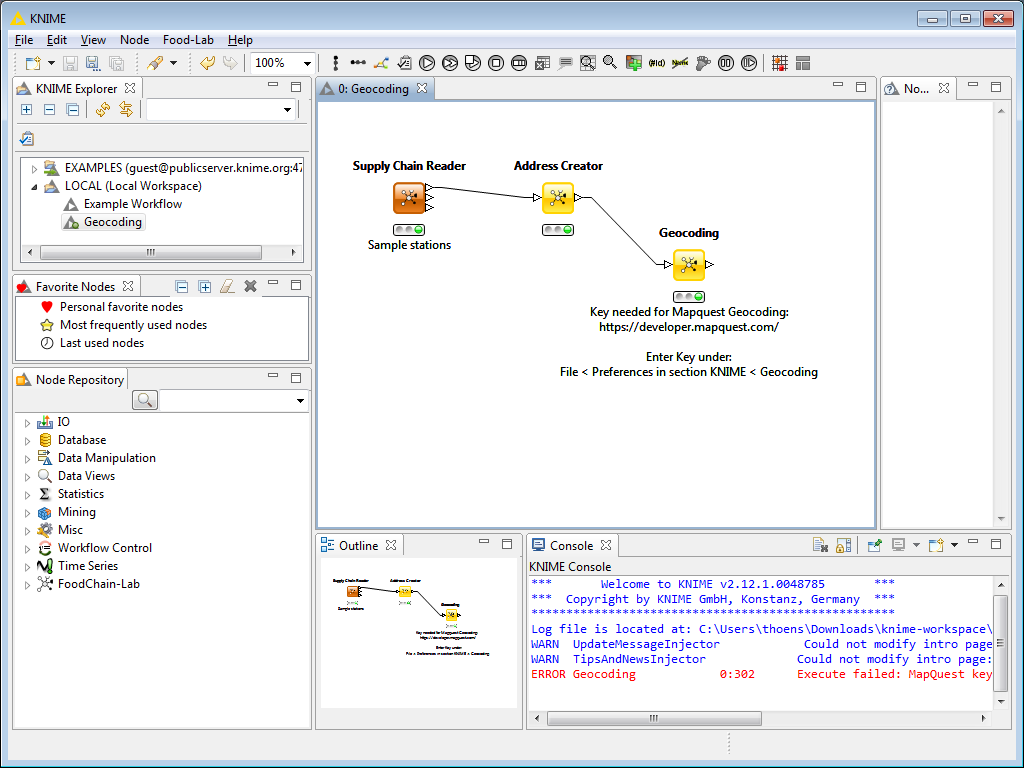
\includegraphics[height=0.6\textheight]{1.png}
	\end{center}
	\begin{itemize}
		\item Import the Geocoding workflow from \url{https://github.com/SiLeBAT/BfROpenLabResources/raw/master/GitHubPages/workflows/Geocoding.zip}.
		\item In this tutorial we are using the MapQuest Open Geocoding service.
	\end{itemize}
\end{frame}

\subsection{2}
\begin{frame}
	\begin{center}
  		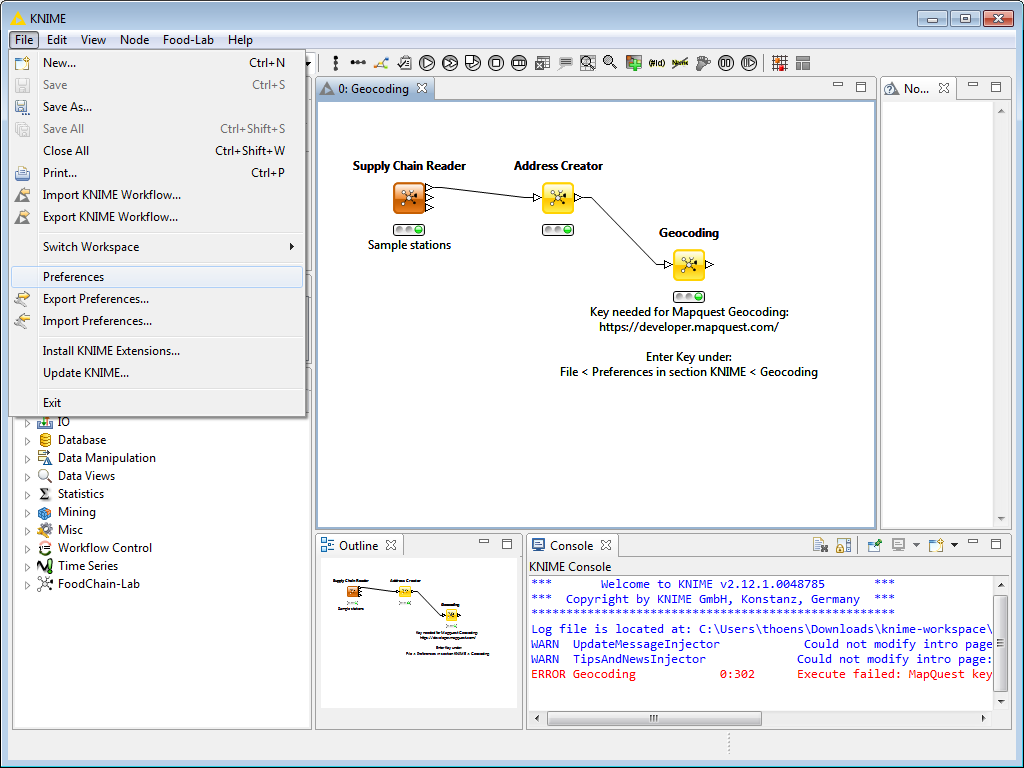
\includegraphics[height=0.6\textheight]{2.png}
	\end{center}
	\begin{itemize}		
		\item For using MapQuest you have to register and create a key at \url{http://developer.mapquest.com/web/info/account/app-keys}
		\item This key has to be entered in the KNIME preferences.
		\item Select \textbf{File $<$ Preferences} in the menu bar.
	\end{itemize}
\end{frame}

\subsection{3}
\begin{frame}
	\begin{center}
  		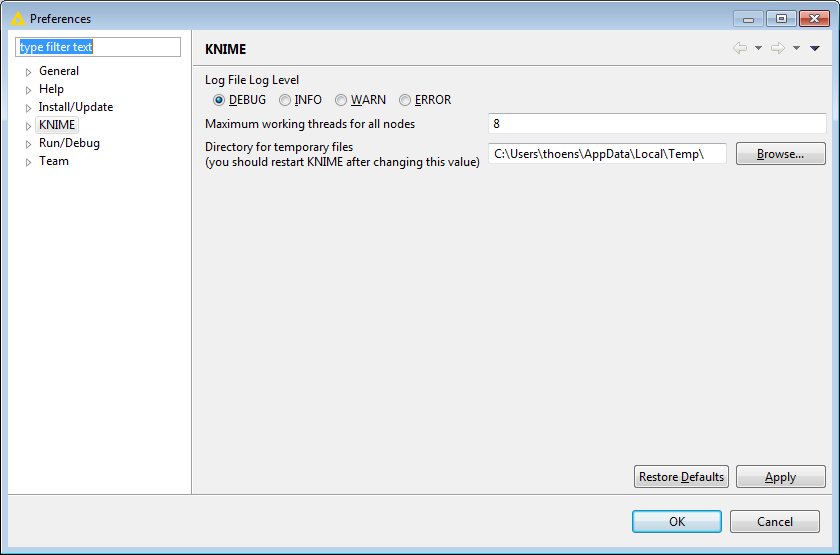
\includegraphics[height=0.6\textheight]{3.png}
	\end{center}
	\begin{itemize}
		\item The Preferences dialog will pop up.
		\item Here you can specify all preferences for KNIME and FoodChain-Lab.
	\end{itemize}
\end{frame}

\subsection{4}
\begin{frame}
	\begin{center}
  		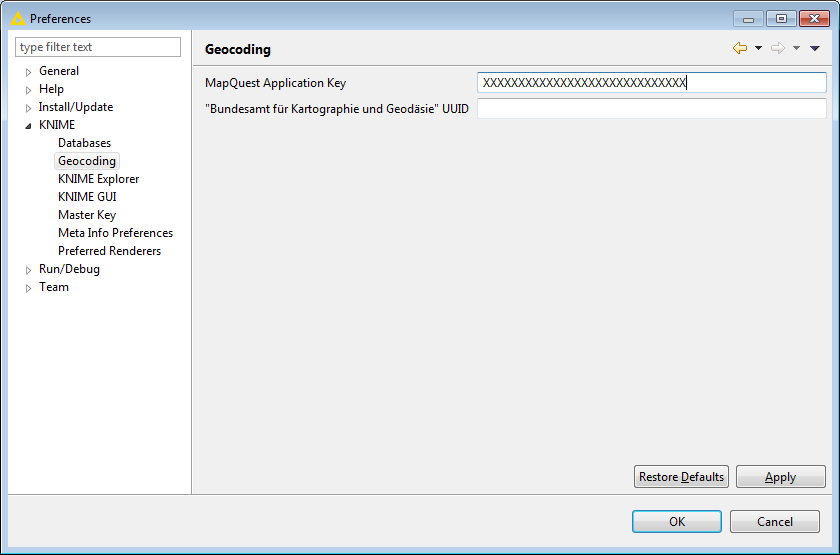
\includegraphics[height=0.6\textheight]{4.png}
	\end{center}
	\begin{itemize}
		\item Select \textbf{KNIME $<$ Geocoding} in the navigation tree on the left.
		\item Enter your \textbf{MapQuest Application Key} and press \textbf{OK}.
	\end{itemize}
\end{frame}

\subsection{5}
\begin{frame}
	\begin{center}
  		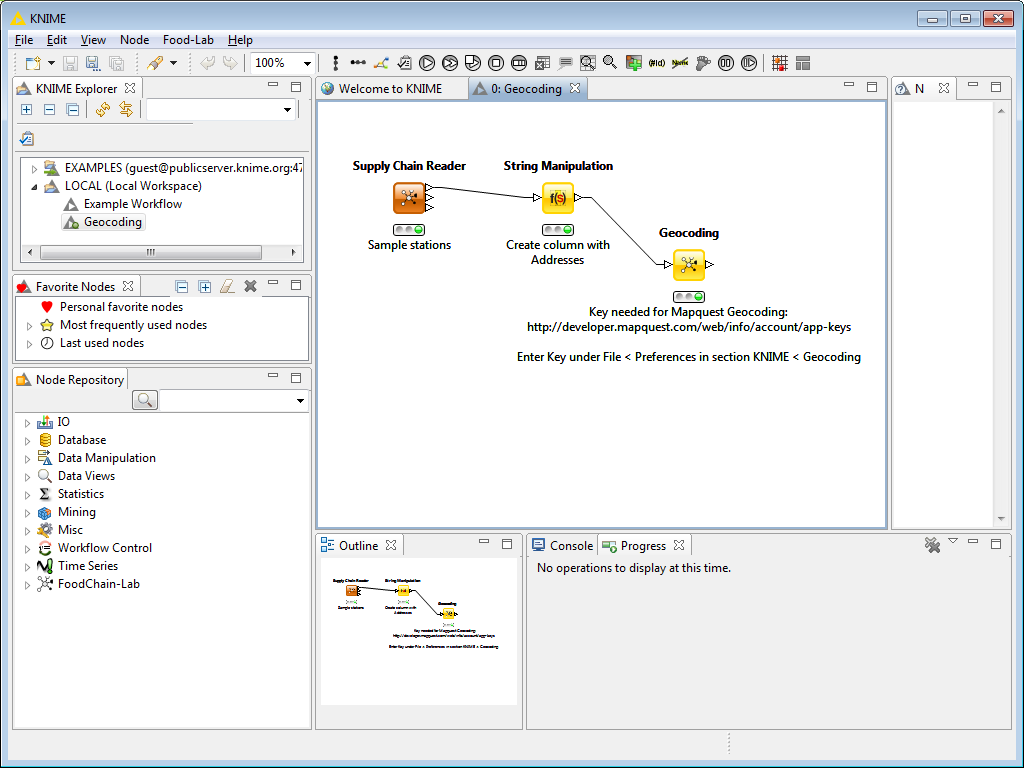
\includegraphics[height=0.6\textheight]{5.png}
	\end{center}
	\begin{itemize}
		\item To perform geocoding we need one column with addresses in our data table. The \textbf{Supply Chain Reader} puts out all parts of the address (street, city, ...) in different columns.
		\item The address column is created in the \textbf{String Manipulation} node.
		\item Double click on this node to open its dialog.
	\end{itemize}
\end{frame}

\subsection{6}
\begin{frame}
	\begin{center}
  		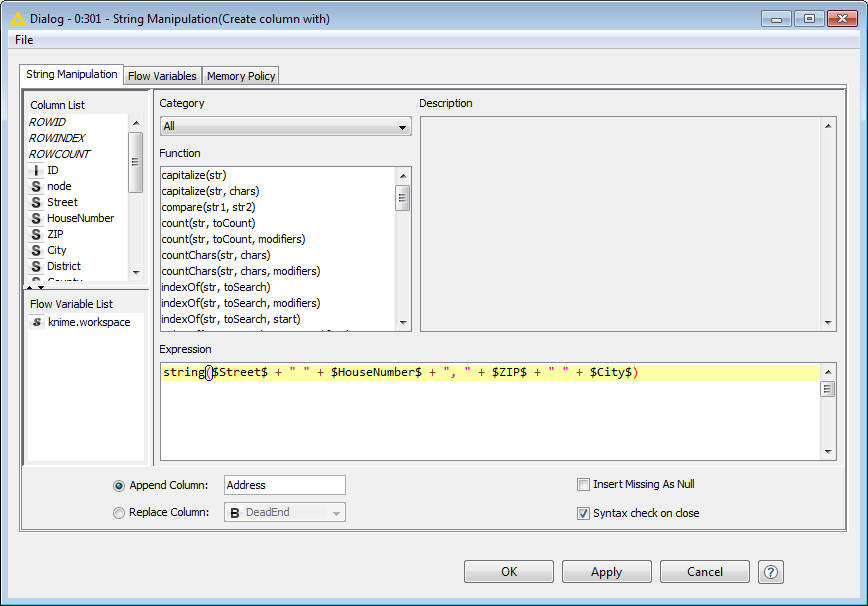
\includegraphics[height=0.6\textheight]{6.png}
	\end{center}
	\begin{itemize}
		\item In the dialog you can provide the name of the address column and an expression, that defines how the address column is created.
		\item We want to change this expression, so that the zip code is not used anymore.	
	\end{itemize}
\end{frame}

\subsection{7}
\begin{frame}
	\begin{center}
  		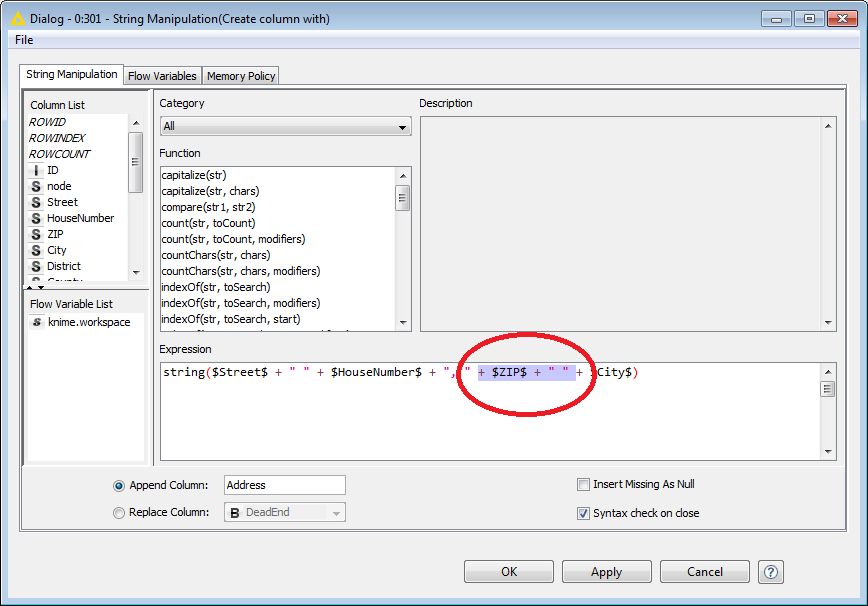
\includegraphics[height=0.6\textheight]{7.png}
	\end{center}
	\begin{itemize}
		\item To remove the zip code we have to remove all characters with a purple background.
		\item These characters include the zip code itself and the space between zip code and city.
	\end{itemize}
\end{frame}

\subsection{8}
\begin{frame}
	\begin{center}
  		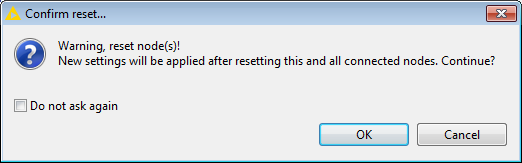
\includegraphics[height=0.6\textheight]{8.png}
	\end{center}
	\begin{itemize}
		\item Now we want to add the country to the expression.
		\item \textbf{Country} and all other columns are available in the \textbf{Columm List} on the left.
	\end{itemize}
\end{frame}

\subsection{9}
\begin{frame}
	\begin{center}
  		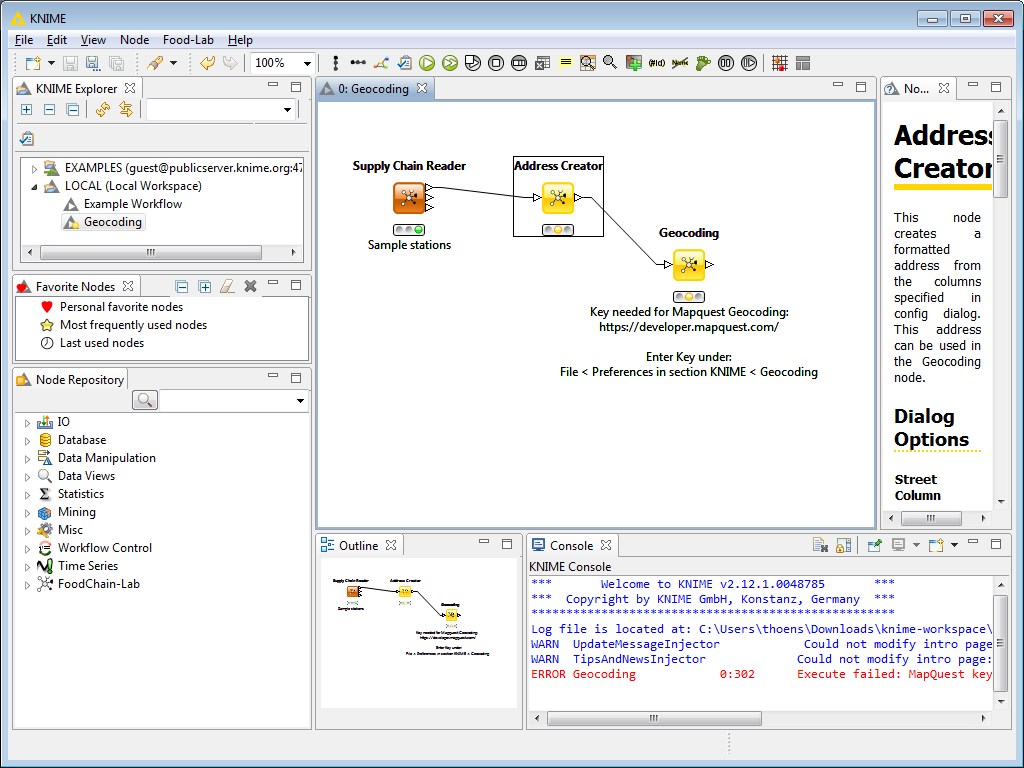
\includegraphics[height=0.6\textheight]{9.png}
	\end{center}
	\begin{itemize}
		\item After \textbf{\$City\$} enter the following: \textbf{+ ", " +}
		\item Then double click on \textbf{Country} in the \textbf{Column List} and the expression should look like this.
		\item Press \textbf{OK} to close the dialog.
	\end{itemize}
\end{frame}

\subsection{10}
\begin{frame}
	\begin{center}
  		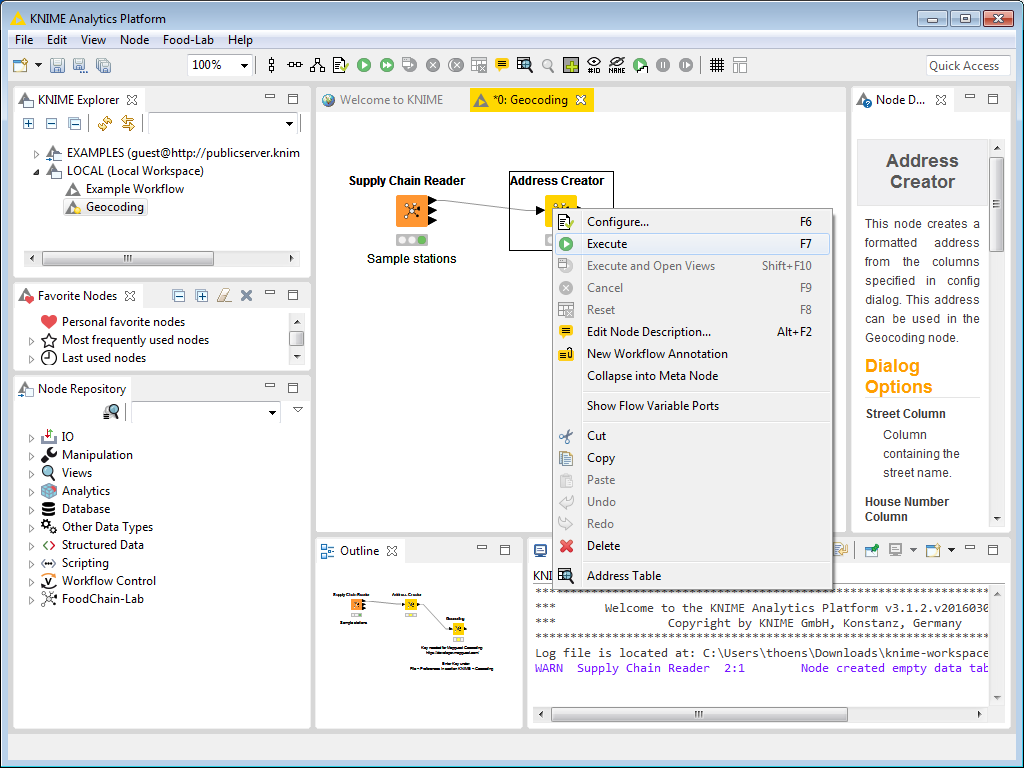
\includegraphics[width=0.9\textwidth]{10.png}
	\end{center}
	\begin{itemize}
		\item Since we changed the settings, the node has to be reset.
		\item Press \textbf{OK}.
	\end{itemize}
\end{frame}

\subsection{11}
\begin{frame}
	\begin{center}
  		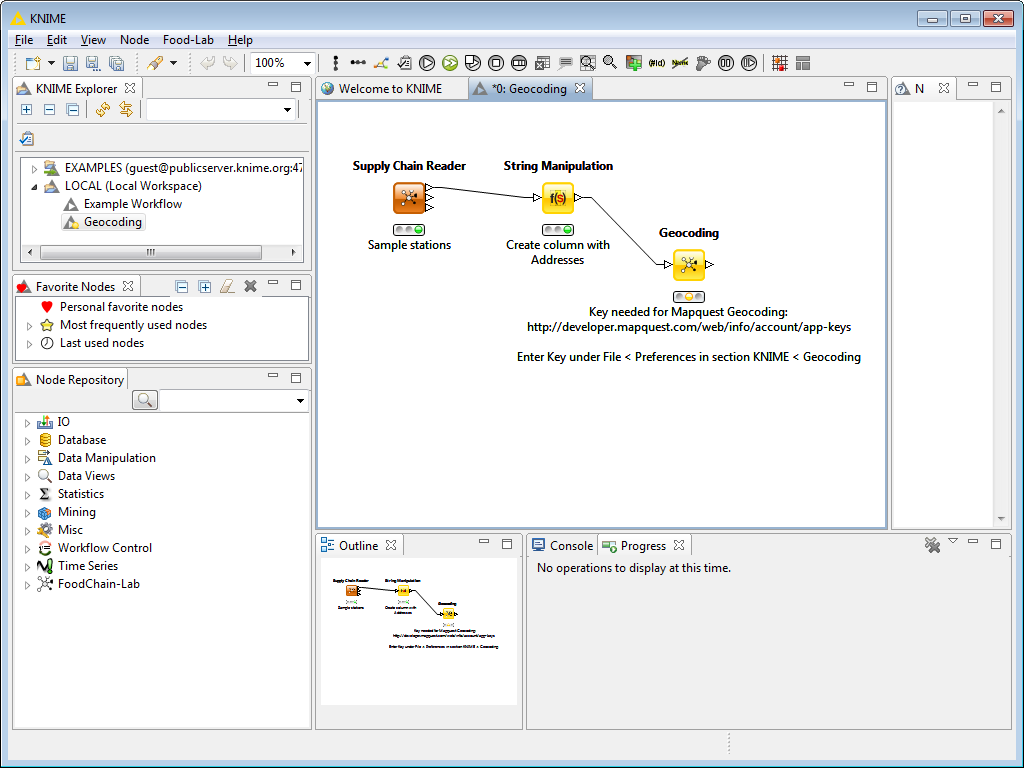
\includegraphics[height=0.6\textheight]{11.png}
	\end{center}
	\begin{itemize}
		\item The expression for the \textbf{Address} column has been updated in the \textbf{String Manipulation} node.
	\end{itemize}
\end{frame}

\subsection{12}
\begin{frame}
	\begin{center}
  		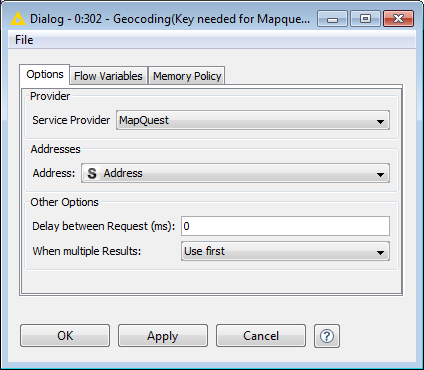
\includegraphics[height=0.6\textheight]{12.png}
	\end{center}
	\begin{itemize}
		\item Right click on the \textbf{String Manipulation} node and select \textbf{Execute}.
	\end{itemize}
\end{frame}

\subsection{13}
\begin{frame}
	\begin{center}
  		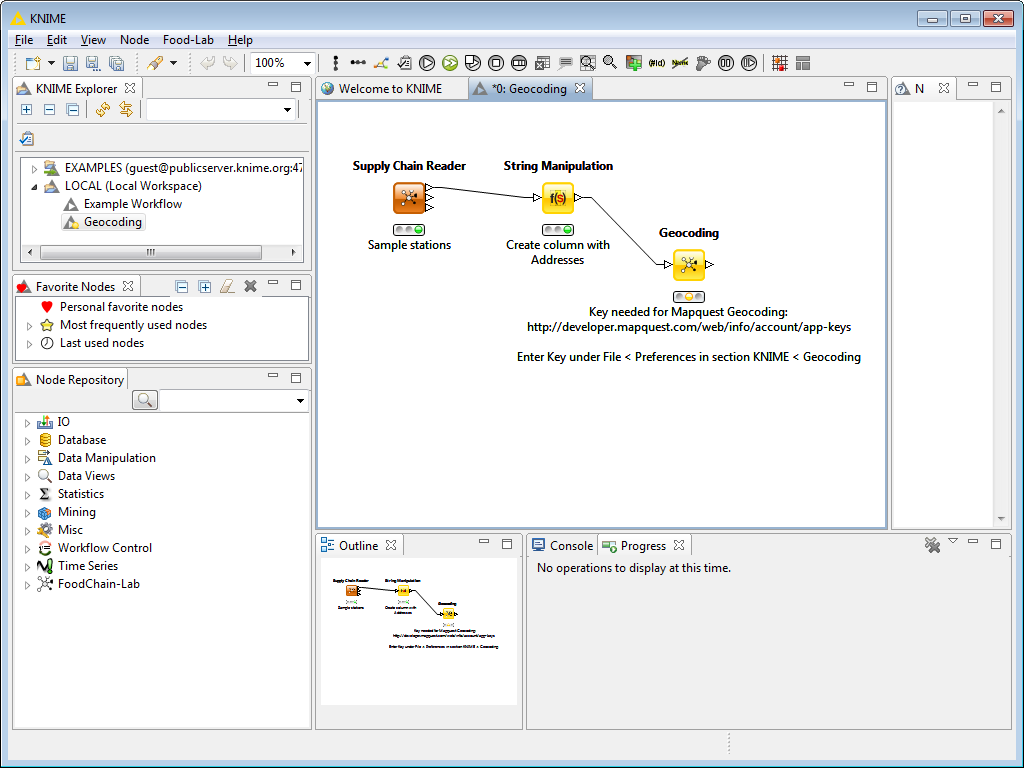
\includegraphics[height=0.6\textheight]{13.png}
	\end{center}
	\begin{itemize}
		\item Now that we updated the \textbf{Address}, the geocoding can be set up.
		\item Double click on the \textbf{Geocoding} node to open its dialog.
	\end{itemize}
\end{frame}

\subsection{14}
\begin{frame}
	\begin{center}
  		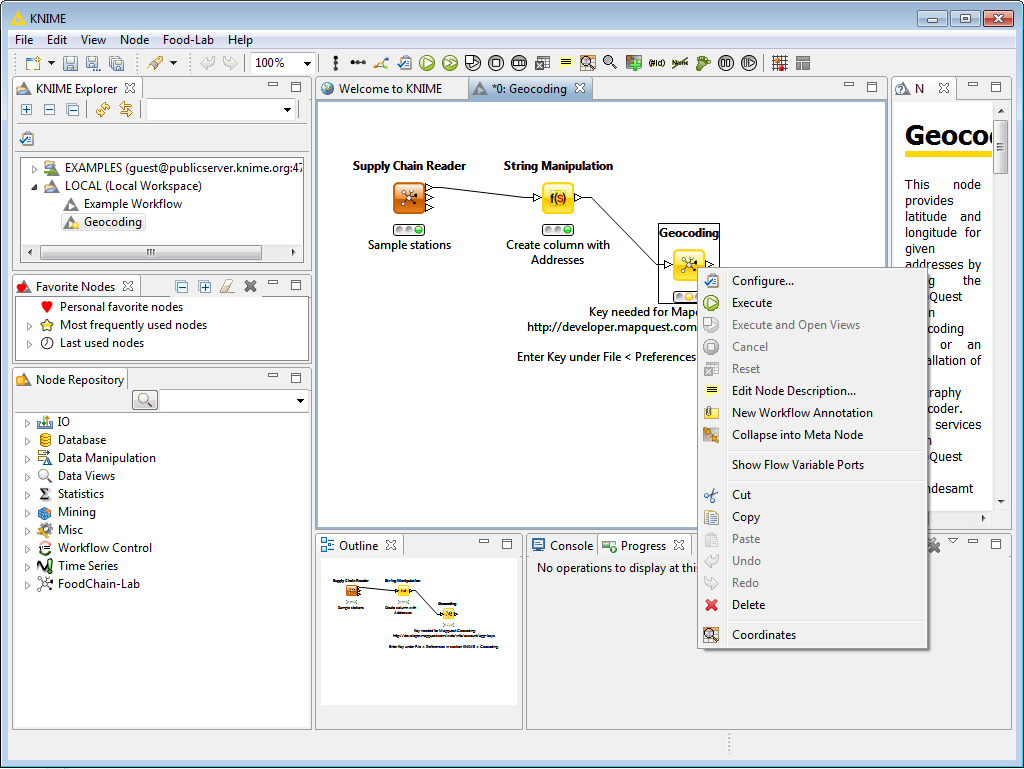
\includegraphics[height=0.6\textheight]{14.png}
	\end{center}
	\begin{itemize}
		\item Here you can specify the \textbf{Service Provider} for geocoding and the column that should be used.
		\item Both are already correct, so we don't need to change anything here.
	\end{itemize}
\end{frame}

\subsection{15}
\begin{frame}
	\begin{center}
  		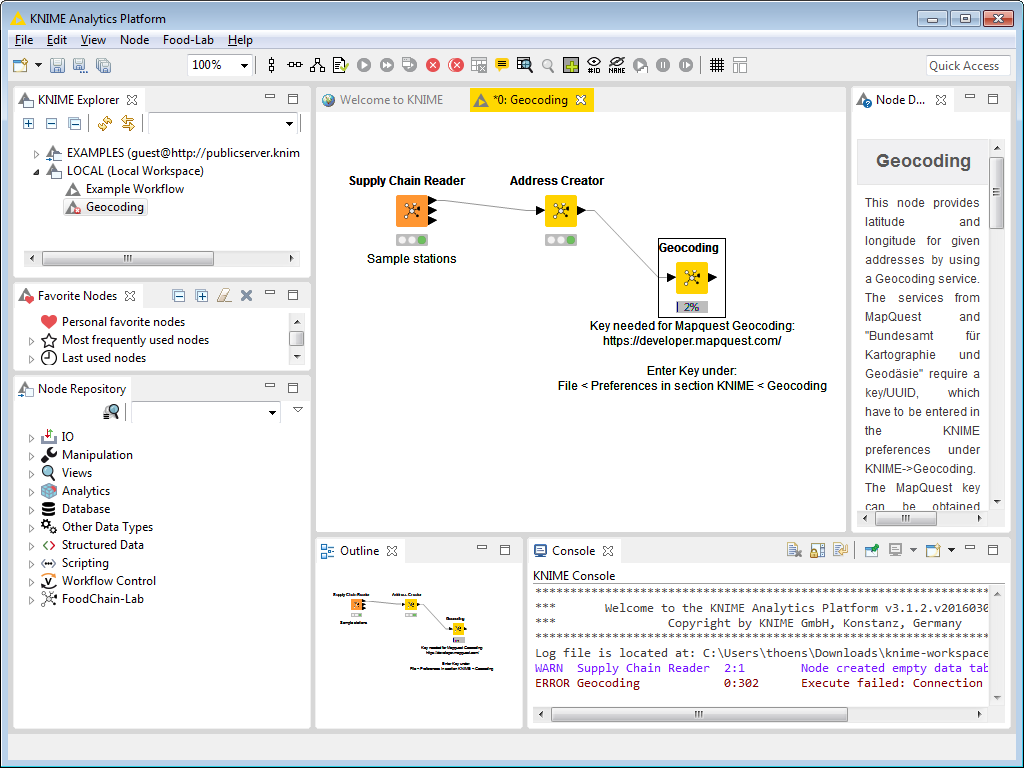
\includegraphics[height=0.5\textheight]{15.png}
	\end{center}
	\begin{itemize}
		\item For many request geocoding services return multiple results (e.g. when there are two streets with the same name).
		\item To deal with this we have to decide if we just want to use the first or look at all choices and try to find the best.
		\item Looking manually at all choices is a lot of work for large data sets, so just select \textbf{Use first} and press \textbf{OK}.
	\end{itemize}
\end{frame}

\subsection{16}
\begin{frame}
	\begin{center}
  		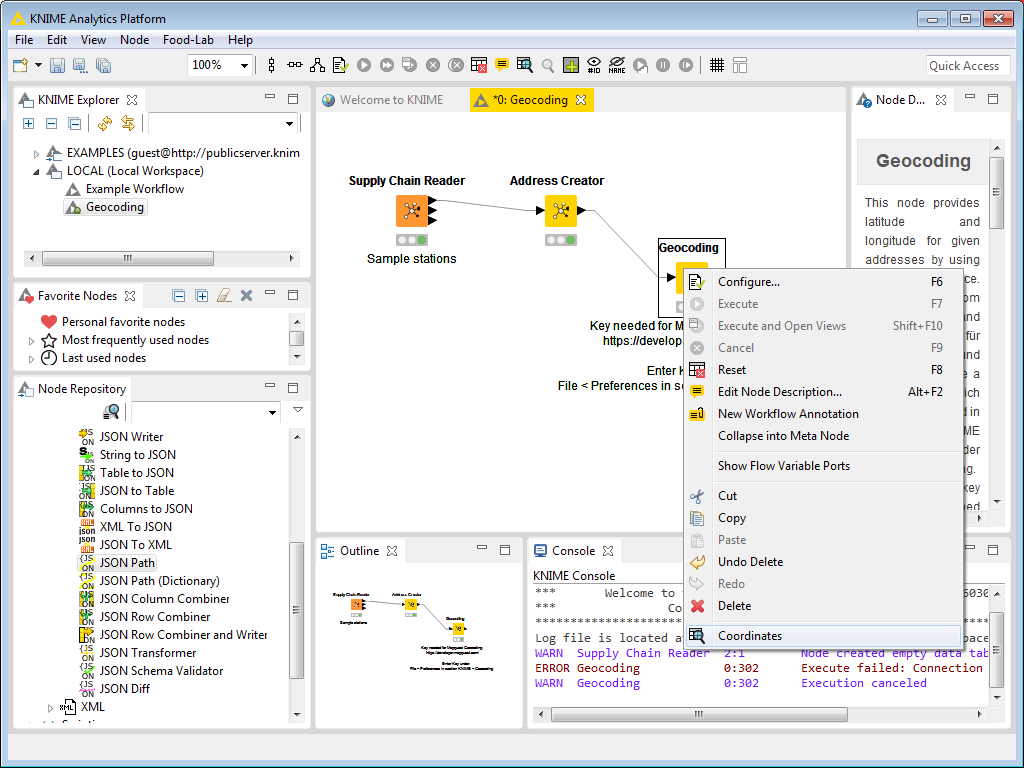
\includegraphics[height=0.6\textheight]{16.png}
	\end{center}
	\begin{itemize}
		\item Right click on the \textbf{Geocoding} node and select \textbf{Execute}.
	\end{itemize}
\end{frame}

\subsection{17}
\begin{frame}
	\begin{center}
  		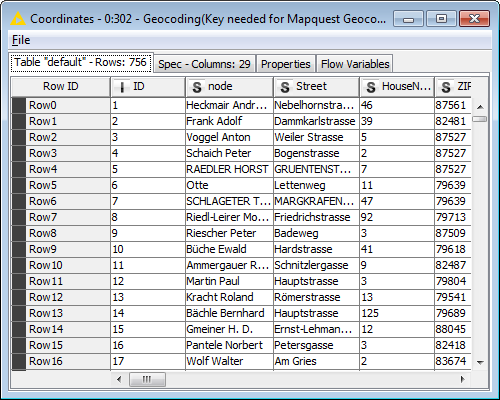
\includegraphics[height=0.6\textheight]{17.png}
	\end{center}
	\begin{itemize}
		\item The execution can take a while.
		\item The progress bar under the node shows what percentage of data has been processed.
	\end{itemize}
\end{frame}

\subsection{18}
\begin{frame}
	\begin{center}
  		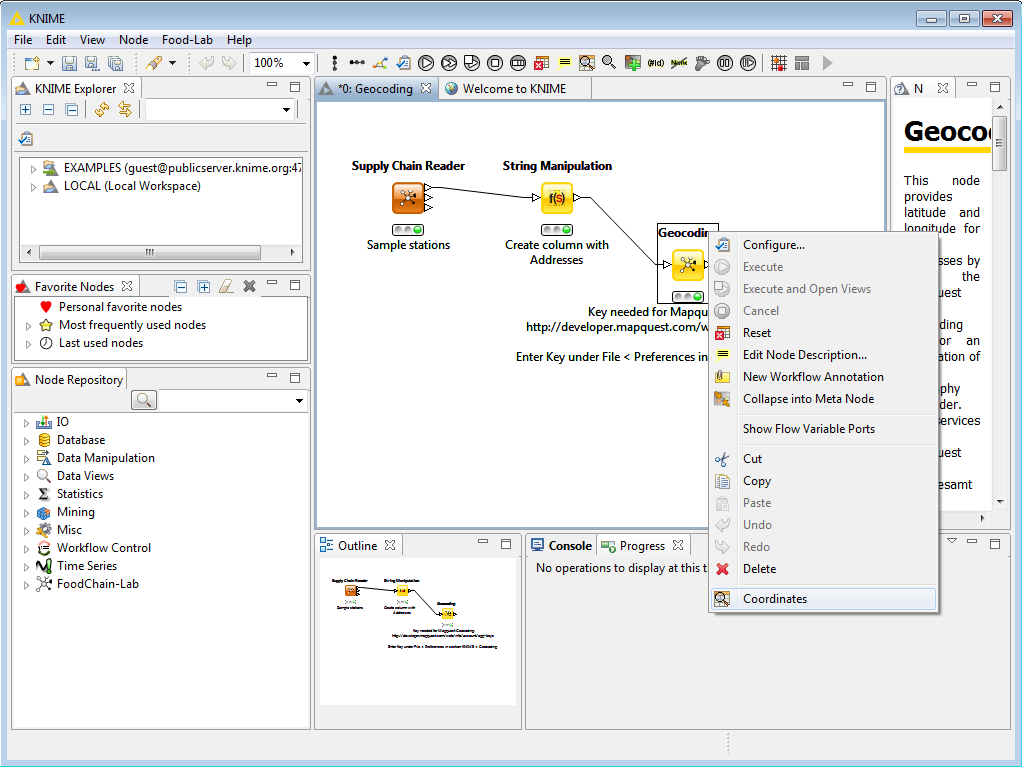
\includegraphics[height=0.6\textheight]{18.png}
	\end{center}
	\begin{itemize}
		\item When the execution is finished, we can look at the results.
		\item Right click on the \textbf{Geocoding} node and select \textbf{Coordinates}.
	\end{itemize}
\end{frame}

\subsection{19}
\begin{frame}
	\begin{center}
  		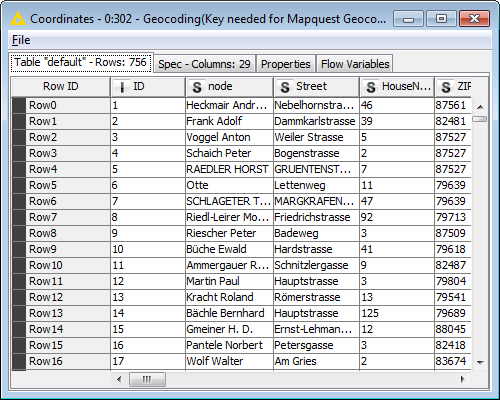
\includegraphics[height=0.6\textheight]{19.png}
	\end{center}
	\begin{itemize}
		\item In the dialog that pops up, you can look at the whole data table.
	\end{itemize}
\end{frame}

\subsection{20}
\begin{frame}
	\begin{center}
  		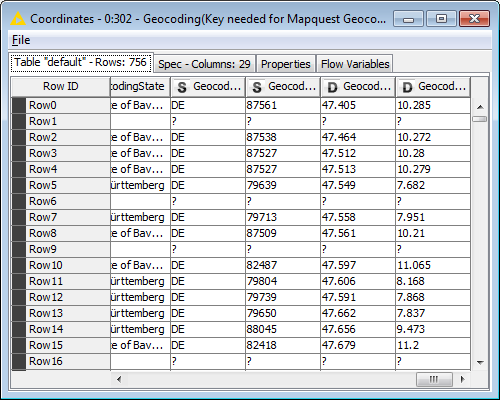
\includegraphics[height=0.6\textheight]{20.png}
	\end{center}
	\begin{itemize}
		\item Scroll to the right to look at the columns with latitude and longitude (the two rightmost columns).
		\item For all rows with "?" the geocoding was unsuccessful.
	\end{itemize}
\end{frame}

\end{document}